\documentclass[a4paper,12pt]{article}
\usepackage[utf8]{inputenc} 
\usepackage{graphicx} 
\usepackage{lmodern} 
\usepackage{cite}
\usepackage{hyperref}
\usepackage{array}
\usepackage{listings}
\usepackage{color}
\hypersetup{%
    pdfborder = {0 0 0}
}

\usepackage[top = 3cm, left = 2.5cm, bottom = 2.5cm, right = 2.5cm]{geometry}
\lstset{language=sql, basicstyle=\small\ttfamily, breaklines,prebreak= , postbreak= , frame=shadowbox, keywordstyle=\color{red}}

\begin{document}
 
\setlength{\parindent}{0cm}
\setlength{\parskip}{1ex plus 0.5ex minus 0.2ex}
\newcommand{\hsp}{\hspace{20pt}}
\newcommand{\HRule}{\rule{\linewidth}{0.5mm}}
\begin{titlepage}
  \begin{sffamily}
  \begin{center}

    
\includegraphics[scale=0.2]{logo.jpg}\\[2cm]

    \textsc{\LARGE Université de Nantes}\\
    \textsc{\LARGE  }\\
    \textsc{\Large UFR Sciences et Techniques}\\
    \textsc{\LARGE  }\\
 	[1.5cm]
    % Title
    \HRule \\[0.4cm]
    { \huge \bfseries Bases de données - niveau 2 \\[0.4cm]
    	
     }
     \textsc{\Large XOIB040}\\
    \HRule \\[1cm]

    % Author and supervisor
    
    
    
\includegraphics[scale=0.8]{image.jpg}
      \vfill
      \begin{center} \large
       Ulysse \textsc{Guyet}\\
       Jennifer \textsc{Rondineau}\\
       \end{center}
       \begin{center} \large
       Master 2 Bioinformatique \\
       \end{center}
      

   

    % Bottom of the page
    {\large 2 mars 2016}

  \end{center}
  \end{sffamily}
\end{titlepage}
 % page de garde
\renewcommand{\contentsname}{Sommaire} 
\tableofcontents{} 
\clearpage


 \textbf{Conception d'une base de données, capable de suivre l'emprunt de libres par les membres d'une bibliothèque. }

Dans un premier temps, nous avons défini les tables nécessaires pour stocker les informations de la bibliothèques :

    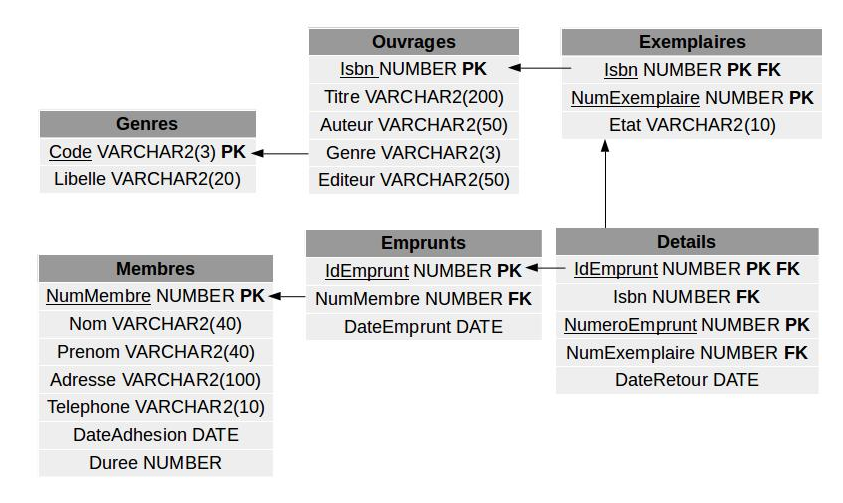
\includegraphics[scale=0.5]{tables.png} 

 \textbf {PK} : clé primaire\\
 \textbf {FK} : clé étrangère


\section{Langage de définition de données}
 \textbf {1)} Nous avons créé nos tables avec les instructions "CREATE TABLE", en prenant en compte les contraintes d'intégrités décrites ci-dessus sur le schéma représentant les tables de notre base. 
 
  La table \textbf {Genres} a comme clé primaire le "code" à 3 lettres du genre.
  
 La table \textbf {Ouvrages} a comme clé primaire l'identifiant "isbn", et comme clé étrangère "genre" qui fait réference au "code" de la table Genres. 
 
 La table \textbf {Exemplaire}s a comme clé primaire l'isbn et le numéro de l'exemplaire. L'isbn est une clé étrangère qui reference la table Ouvrage. 
 
 La table \textbf {Membres} a comme clé primaire le numéro de membre. 
 
 La table \textbf {Emprunts} a comme clé primaire le numéro d'identification de l'emprunt (idEmprunt), et comme clé étrangère le numéro du membre qui réalise l'emprunt, clé étrangère qui référence la table Membres. 
 
 La table \textbf {Détails} a comme clé primaire le numéro d'identification de l'emprunt (idEmprunt) et le numéro de l'emprunt (NumeroEmprunt). Les clés étrangères de cette table sont : isbn et le numero de l'exemplaire qui font référence à la table Exemplaire et l'idEmprunt qui référence la table Emprunt.\\
 
 
\textbf {2) }
 \begin{lstlisting}
 CREATE SEQUENCE incrementation START WITH 1 INCREMENT BY 1;
 \end{lstlisting}
Cette séquence "incrementation" va nous permettre de pouvoir numéroté automatiquement le numéro d'identifiant des membres et le numéro d'identification des emprunts. Cette séquence permet d'incrémenter par 1, un compteur commençant à 1. \\

\textbf {3) }
 \begin{lstlisting}
ALTER TABLE Membres ADD CONSTRAINT unique_membres UNIQUE(nom, prenom, telephone);
 \end{lstlisting}

Cette commande permet d'ajouter une contrainte sur la table Membres, l'instruction "UNIQUE" permet que deux membres de la bibliothèques ne peuvent pas avoir le même nom, prénom et numéro de téléphone. Nous avons nommé cette contrainte "unique\_membres".\\

\textbf {4) }
 \begin{lstlisting}
ALTER TABLE Membres ADD portable CHAR(10) CONSTRAINT check_06 CHECK (portable LIKE '06%');
  \end{lstlisting}

Cette commande permet d'ajouter une colonne "portable" à la table des Membres, un numéro de téléphone étant une suite de 10 numéros, on définit cette variable comme étant un CHAR(10), et on ajoute une contrainte nommé "check\_06" qui vérifie que le numéro de portable commence bien par 06 (LIKE 'O6 \%').\\

\textbf {5) } On souhaite supprimer la colonne telephone, comme la plupart des étudiants ne disposent que d'un numéro de téléphone portable, on souhaite garder que celui-ci. Le téléphone fait partie d'une contrainte d'unicité dans la table Membres. Il faut tout d'abord commencer par supprimer cette contrainte : 
 \begin{lstlisting}
ALTER TABLE Membres DROP CONSTRAINT unique_membres;
\end{lstlisting}
Puis, on crée une nouvelle contrainte, mais cette fois ci, avec le numéro de téléphone portable : 
 \begin{lstlisting}
ALTER TABLE Membres ADD CONSTRAINT unique_membres UNIQUE(nom, prenom, portable); 
\end{lstlisting}
Il est important de ne pas apporter de grande modification sur la base pendant les heures d'ouvertures de la bibliothéques, donc en attendant de pouvoir supprimer la colonne "téléphone", on commence par la rendre inutilisable :
 \begin{lstlisting}
ALTER TABLE Membres SET UNUSED(telephone);
\end{lstlisting}

Lorsque la charge de travail sera plus faible on pourra alors supprimer ces données : 
 \begin{lstlisting}
ALTER TABLE Membres DROP UNUSED COLUMNS;
\end{lstlisting}
Cette commande permet de supprimer toutes les données rendues inutilisables. 

\textbf {6) }
Pour améliorer les performance d'accès aux données, on définit un index sur toutes les colonne de type clé étrangère, afin de rendre les opérations de jointure plus rapides : 
 \begin{lstlisting}
CREATE INDEX index_FK_exemplaires_isbn ON Exemplaires(isbn);
CREATE INDEX index_FK_Emprunts_numMembre ON Emprunts(numMembre);
CREATE INDEX index_FK_idEmprunt ON DetailsEmprunts(idEmprunt);
CREATE INDEX index_FK_isbn ON DetailsEmprunts(isbn);
CREATE INDEX index_FK_numExemplaire ON DetailsEmprunts(numExemplaire);
\end{lstlisting}

\textbf {7) } A l’usage, on se rend compte que lorsque l’on souhaite supprimer une fiche d’emprunt, il faut nécessairement supprimer toutes les lignes précédentes dans la table 'DETAILSEMPRUNTS' qui font référence à la table 'EMPRUNTS' que l’on souhaite supprimer. 

Il est possible de rendre automatique une telle suppression en ajoutant aux clés étrangères une contrainte 'ON DELETE CASCADE' qui permettra de supprimer toutes les références. 
 \begin{lstlisting}
ALTER TABLE DetailsEmprunts DROP CONSTRAINT fk_idemprunt;
ALTER TABLE DetailsEmprunts ADD CONSTRAINT fk_idemprunt FOREIGN KEY (idEmprunt) REFERENCES Emprunts(idEmprunt) ON DELETE CASCADE ;
\end{lstlisting}

On supprime d'abord l'ancienne contrainte de la clé étrangère "fk\_idEmprunt" de la table 'DetailsEmprunts' et on ajoute une nouvelle contrainte de clé étrangère contenant 'ON DELETE CASCADE'. 

\textbf {8) }
\begin{lstlisting}
ALTER TABLE Exemplaires MODIFY etat DEFAULT 'NE';
\end{lstlisting}

Cette commande permet de modifier la colonne 'etat' de la table 'Exemplaires', par défaut l'état d'un nouvel exemplaire sera "NE" pour neuf. 

\textbf {9) }
 \begin{lstlisting}
 CREATE SYNONYM Abonnes FOR Membres;
 \end{lstlisting}

Cette commande permet de créer un synonyme "Abonnés" pour la table "Membres", ainsi dans les futures requêtes, il sera possible de faire référence à la table des membres ou bien à la table des abonnés.

\textbf {10) }
 \begin{lstlisting}
ALTER TABLE DetailsEmprunts RENAME TO Details;
 \end{lstlisting}

Cette commande permet de renommer la table 'DetailsEmprunts' par 'Details'. Par la suite, on ne pourra faire référence à cette table que par 'Details'. 

\clearpage

\section{Langage de manipulation de données}

\textbf {1) }Nous avons ajouté dans nos tables, les informations suivantes : 

La table Genres :
\begin{center}
    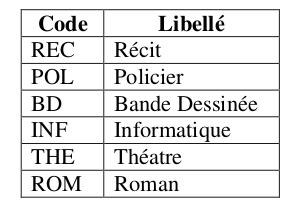
\includegraphics[scale=0.5]{genres.png}
\end{center}
La table Ouvrages : 
\begin{center}
    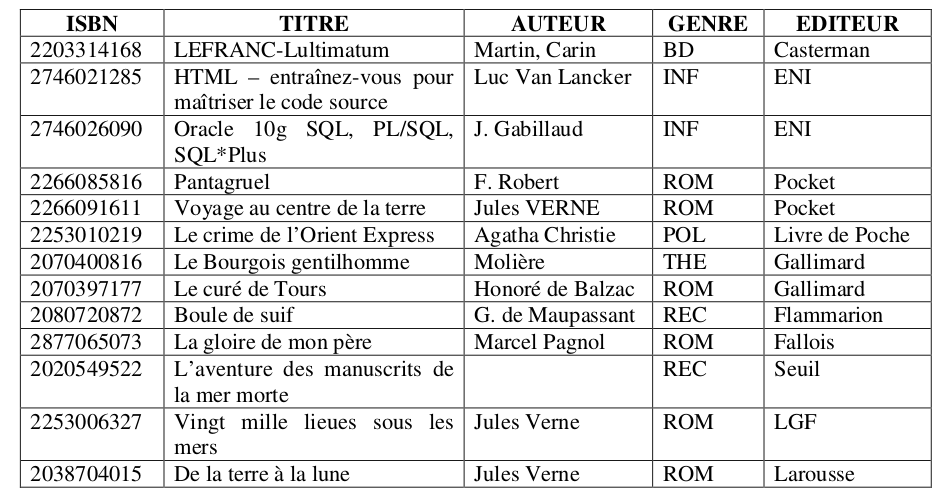
\includegraphics[scale=0.5]{ouvrages.png}
\end{center}

La table Exemplaires : 
\begin{center}
    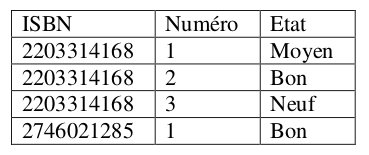
\includegraphics[scale=0.5]{exemplaire.png}
\end{center}

Ces ajouts dans les tables ont été réalisés avec l'instruction 'INSERT INTO'.

\clearpage
\textbf {2) } Pour la table Membres, on affecte un numéro de membre à chaque abonnée grâce à la séquence incrémentation crée précédemment.

\begin{center}
    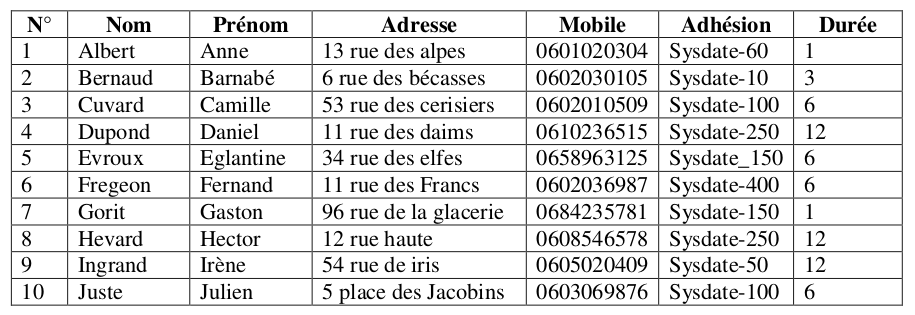
\includegraphics[scale=0.5]{membres.png}
\end{center}
 Par exemple pour le premier membre, nous avons inséré ses données ainsi : 
 \begin{lstlisting}
INSERT INTO Membres VALUES(incrementation.nextval, 'Albert', 'Anne', '13 rue des Alpes', Sysdate-60, 1, '0601020304');
  \end{lstlisting}
 
 Afin que la base de données soit toujours à jour, toutes les données de type date sont exprimées en relatif par rapport à la date du jour du serveur (SYSDATE). Par exemple, SYSDATE-2, correspond à une date antérieur de 2 jour.
 
 \textbf {3) } Nous avons complété de la même façon, la table des Emprunts et des détails des emprunts. 
 
  \textbf {4) Extraction simple d’informations }

Afin de consulter le contenu de chaque, on utilise ces requêtes : 
\begin{lstlisting}
SELECT * FROM Ouvrages;
SELECT * FROM Exemplaires;
SELECT * FROM Membres;
SELECT * FROM Emprunts;
SELECT * FROM Details;
SELECT * FROM Genres;
  \end{lstlisting}
Ceci nous permet de visualiser toutes les lignes et toutes les colonnes de chaque table. 

  \textbf {5) Activation de l’historique des mouvements}
  
Les manipulations de la table des membres et des détails des emprunts sont sensibles, afin d'avoir un suivi des changements réalisés sur ces tables, on active l’historique des mouvements :
\begin{lstlisting}
ALTER TABLE Membres ENABLE ROW MOVEMENT; 
ALTER TABLE DETAILS ENABLE ROW MOVEMENT ;
  \end{lstlisting}
  
  \clearpage
  
    \textbf {6) Ajout d’une colonne :}
    
Afin de faciliter la gestion des emprunts et identifier plus rapidement les fiches pour lesquelles l'ensemble des exemplaires n'est pas restitué, on ajoute une colonne 'etat' à la table emprunt : 
\begin{lstlisting}
ALTER TABLE Emprunts ADD etat char(2) DEFAULT 'EC' ;
\end{lstlisting}
Cette colonne prendra par défaut la valeur 'EC' pour 'En Cours' et sinon 'RE' pour 'Rendue' lorsque l'ensemble des exemplaires est rendu : 
\begin{lstlisting}
ALTER TABLE Emprunts ADD CONSTRAINT check_emprunts CHECK (etat IN('EC','RE'));
\end{lstlisting}
La contrainte 'check\_emprunts' permet d'imposer que cette colonne ne peut prendre comme valeur que 'EC' ou 'RE'. 

Par défaut pour le moment tous les états sont à 'EC', il faut alors mettre à jour l'état de chaque fiche d'emprunt en faisant passer à RE (rendue) l'état si tous les ouvrages empruntés par le membre ont été restitués à la bibliothèques (c'est à dire s'ils ont tous une dateRetour renseignée).

\begin{lstlisting}
UPDATE Emprunts SET etat='RE' WHERE etat='EC' AND idemprunt NOT IN (SELECT idemprunt FROM Details WHERE dateretour IS NULL);
\end{lstlisting}

  \textbf {7) Mise à jour conditionnelle :}

On souhaite modifier l’état des exemplaires en fonction de leur nombre de locations. 

Tout d'abord, nous allons créer une table temporaire 'Locations' permettant de stocker isbn des ouvrages, le numéro d'exemplaire ainsi que le nombre de fois que cet exemplaire a été emprunté :

\begin{lstlisting}
CREATE TABLE Locations AS SELECT isbn, numExemplaire, count(*) AS nblocation FROM Details GROUP BY isbn, numExemplaire;
\end{lstlisting}

Ensuite, on réalise une mise à jour de la table Exemplaires, en modifiant l'état des livres qui ont été emprunté entre 11 et 25, par un "bon" état. 
\begin{lstlisting}
UPDATE Exemplaires SET etat='Bon' WHERE (isbn, numExemplaire) IN (SELECT isbn, numExemplaire FROM Locations WHERE nblocation BETWEEN 11 AND 25);
\end{lstlisting}

Les livres empruntés entre 26 et 60 fois, seront dans un état "moyen" : 
\begin{lstlisting}
UPDATE Exemplaires SET etat='Moyen' WHERE (isbn, numExemplaire) IN (SELECT isbn, numExemplaire FROM Locations WHERE nblocation BETWEEN 26 AND 60);
\end{lstlisting}

Et les exemplaires loués plus de 60 fois seront dans un "mauvais état" : 
\begin{lstlisting}
UPDATE Exemplaires SET etat='Mauvais' WHERE (isbn, numExemplaire) IN (SELECT isbn, numExemplaire FROM Locations WHERE nblocation > 60);
\end{lstlisting}

A partir de là, on peut supprimer tous les livres qui ont un état "mauvais" : 
\begin{lstlisting}
DELETE FROM Exemplaires WHERE etat='Mauvais';
\end{lstlisting}

Et pour finir, dernière étape, on supprime la table temporaire 'Locations' : 
\begin{lstlisting}
DROP TABLE Locations;
\end{lstlisting}

  \textbf {8)} Afin de supprimer tous les exemplaires dont l'état est "mauvais", on s'y prend comme précédemment : 
\begin{lstlisting}
DELETE FROM Exemplaires WHERE etat='Mauvais';
\end{lstlisting}

  \textbf {9)} Pour établir la liste des ouvrages dont dispose la bibliothèque, il suffit de faire une simple extraction d'information de la table Ouvrages : 
\begin{lstlisting}
SELECT * FROM Ouvrages;
\end{lstlisting}

  \textbf {10)} La liste des membres qui ont emprunté un ouvrage depuis plus de deux semaines en indiquant le nom de l’ouvrage, peut être obtenu ainsi : 
  \begin{lstlisting}
SELECT Membres.numMembre, Membres.nom, Membres.prenom, Ouvrages.titre 
FROM Membres, Ouvrages, Emprunts, Details 
WHERE Membres.numMembre = Emprunts.numMembre AND Emprunts.dateEmprunt < Sysdate-14 AND Details.idemprunt=Emprunts.idEmprunt AND Ouvrages.isbn=Details.isbn AND Details.dateRetour IS NULL ;
   \end{lstlisting}

Cette commande permet de réaliser une jointure entre les tables 'Membres, 'Ouvrages', 'Emprunts' et 'Details'. On sélectionne seulement les membres ayant emprunté un ouvrage depuis plus de deux semaines (SYSDATE-14 : 14 jours soit 2 semaines avant la date du jour), et qui n'ont pas rendu cet ouvrage (dateRetour IS NULL). 


  \textbf {11)} Afin d'établir le nombre d’ouvrages dont on dispose par catégorie, on utilise cette commande : 

\begin{lstlisting}
SELECT genre, count(*) AS NombreOuvrage 
FROM Ouvrages, Exemplaires 
WHERE Ouvrages.isbn=Exemplaires.isbn 
GROUP BY genre; 
\end{lstlisting}
 
Cette commande permet une jointure entre les tables Ouvrages et Exemplaires. L'instruction 'COUNT()' permet de compter le nombre d'ouvrage par genre. Et l'instruction 'GROUP BY' permet de donner le résultat par ordre alphabétique des genres. 
\clearpage
Voici le tableau que nous obtenons : 

\begin{tabular}{ l | c }
   Genres & Nombre d'ouvrages \\
   THE & 2 \\
   INF & 4 \\
   ROM & 12 \\
   BD & 3 \\
   REC & 4 \\
   POL & 2 \\
 \end{tabular}

  \textbf {12)} La durée moyenne d’emprunt d’un livre par un membre se mesure ainsi : 
\begin{lstlisting}
SELECT AVG(dateRetour - DateEmprunt) AS DureeMoyenne 
FROM Emprunts, Details 
WHERE Emprunts.idEmprunt=Details.idEmprunt AND dateRetour IS NOT NULL;
\end{lstlisting}

On réalise une jointure entre les tables Emprunts et Détails. On sélectionné seulement les livres empruntés qui ont été rendus (dateRetour IS NOT NULL), et on effectue une moyenne (AVG()) entre la date de retour du livre et la date à laquelle il a été emprunté.

On obtient une durée moyenne d'emprunt de 13.928 jours.  

  \textbf {13)} La durée moyenne de l’emprunt en fonction du genre du livre se calcule ainsi : 
\begin{lstlisting}
SELECT genre, AVG(dateRetour - DateEmprunt) AS DureeMoyenne
FROM Emprunts, Details, Ouvrages 
WHERE Emprunts.idEmprunt=Details.idEmprunt AND dateRetour IS NOT NULL AND Details.isbn=Ouvrages.isbn GROUP BY genre;
\end{lstlisting}
On réalise une jointure entre les tables Emprunts, Details et Ouvrages. Comme précédemment, on sélectionne les ouvrages qui ont été rendus, et on réalise une moyenne en fonction de leur date d'emprunt et de retour. On regroupe le résultat par genre de livre. Voici le résultat obtenu : 

\begin{tabular}{ l | c }
Genres & Durée moyenne \\
INF  & 19.0002662 \\
ROM  & 13.7859805\\
REC &  13.6669329\\
BD  &  10.0002662\\
POL &   9.0002662\\
 \end{tabular}

  \textbf {14)} Pour établir la liste des ouvrages loués plus de 10 fois au cours des 12 derniers mois, nous devons faire une jointure sur la table des Emprunts, la table contenant les détails des Emprunts et la table des Exemplaires. 
\begin{lstlisting}
SELECT Exemplaires.isbn 
FROM Emprunts, Details, Exemplaires 
WHERE Details.numExemplaire=Exemplaires.numExemplaire AND Details.isbn=Exemplaires.isbn AND Details.idEmprunt=Emprunts.idEmprunt AND MONTHS_BETWEEN(Emprunts.DateEmprunt, Sysdate)<12 
GROUP BY Exemplaires.isbn 
HAVING COUNT(*)>10;
\end{lstlisting}

L'instruction "MONTHS\_BETWEEN(Emprunts.DateEmprunt, Sysdate) \textless 12" permet de sélectionner les emprunts effectués dans les 12 mois précédant la date du jour (sysdate). 

Les ouvrages loués plus de 10 fois sont sélectionnés grâce à l'instruction 'HAVING COUNT(*)$>$10;'. Et le résultat est groupé par numéro d'isbn. 

Pour l'instant dans notre base de données, nous avons aucun ouvrage loués plus de 10 fois au cours des 12 derniers mois. 

  \textbf {15)} Pour établir  la  liste  de  tous  les  ouvrages  associés à leur numéro d’exemplaire existant dans la base, nous avons fait une jointure entre les tables Ouvrages et Exemplaires, et nous sélectionnons toutes les informations de l'ouvrage ainsi que les numéros d'exemplaires : 

  \begin{lstlisting}
  SELECT Ouvrages.*, Exemplaires.numExemplaire 
  FROM Ouvrages, Exemplaires 
  WHERE Ouvrages.isbn=Exemplaires.isbn;
  \end{lstlisting}

Nous obtenons une liste de 27 ouvrages et numéros d'exemplaires. 
  
  \textbf {16)} Pour cette question, on doit définir une vue 'OuvragesEmpruntes' qui permet de connaître pour chaque membre, le nombre d'ouvrages empruntés non rendu. Pour la création de la vue, nous avons utilisé l'instruction "CREATE  [OR REPLACE] VIEW"; et nous avons fait une jointure entre la table des Emprunts et des Détails afin de récupérer les numéros de membres et d'emprunt n'ayant pas de "dateRetour" de renseigné :  

  \begin{lstlisting}
  CREATE OR REPLACE VIEW OuvragesEmpruntes 
  AS SELECT Emprunts.numMembre, COUNT(*) AS NombreLivresEmpruntes 
  FROM Emprunts, Details 
  WHERE Details.idEmprunt=Emprunts.idEmprunt AND Details.dateRetour IS NULL 
  GROUP BY Emprunts.numMembre;
\end{lstlisting}

Nous avons trié le résultat en fonction des numéros de membres. 

  \textbf {17)}
   Pour cette question, nous devons créer une vue ("EmpruntsParOuvrage") qui permet de connaître le nombre d’emprunts par ouvrage. L'instruction "COUNT(*)", nous permet de compter le nombre de fois qu'un ouvrage apparaît dans la table Détails des emprunts. Nous avons regroupé les résultats en fonction de l'isbn de l'ouvrage. 
 \begin{lstlisting}
 CREATE OR REPLACE VIEW EmpruntsParOuvrage 
 AS SELECT isbn, COUNT(*) AS NbEmprunts 
 FROM Details 
 GROUP BY isbn;
 \end{lstlisting}
 
 
   \textbf {18)} 
   Pour établir la liste des membres triés par ordre    alphabétique, on sélectionne tous les membres dans la table Membres et on utilise l'instruction "ORDER BY" qui par défaut trie par ordre alphabétique : 
   \begin{lstlisting}
   SELECT * 
   FROM Membres 
   ORDER BY nom, prenom;
   \end{lstlisting}
   
 \clearpage
 
  \textbf {19)}
  On souhaite obtenir le nombre de locations par titre et le nombre de locations de chaque exemplaire.  
  
  Pour  obtenir  un  tel  résultat,  il  nous est dit qu'il est préférable  d’utiliser  une  table  temporaire  globale et de la  remplir  au  fur  et  à  mesure; en utilisant la  clause  ON  COMMIT  PRESERVE  ROWS  lors  de  la création de la table temporaire globale.
  
  Création de la table temporaire nommé ' EmpruntsResume' contenant l'isbn des ouvrages, le numéro de l'exemplaire, le nombre de location de l'exemplaire et le nombre de location de l'ouvrage : 
  
     \begin{lstlisting}
     CREATE GLOBAL TEMPORARY TABLE EmpruntsResume(
     	isbn NUMBER,
     	numExemplaire NUMBER,
     	NbEmpruntsExemplaire NUMBER,
     	NbEmpruntsOuvrage NUMBER
     )ON COMMIT PRESERVE ROWS;
     \end{lstlisting}
     
 Ensuite, on insère les données concernant les exemplaires dans la table temporaire :      
        \begin{lstlisting}
     INSERT INTO EmpruntsResume(isbn, numExemplaire, NbEmpruntsExemplaire)
     SELECT isbn, numExemplaire, COUNT(*)
     FROM Details
     GROUP BY isbn, numExemplaire;
          \end{lstlisting}

Puis, on insère les données concernant les ouvrages dans la table temporaire : 
    \begin{lstlisting}
     UPDATE EmpruntsResume
     SET NbEmpruntsOuvrage=(SELECT COUNT(*)
     FROM Details
     WHERE Details.isbn=EmpruntsResume.isbn);
     \end{lstlisting}   
     
On termine la mise à jour, en réalisant un commit : 
     \begin{lstlisting}
     COMMIT;
      \end{lstlisting} 

On peut voir le résultat en utilisant la commande "SELECT * FROM EmpruntsResume". 

On supprime la table temporaire : 
    \begin{lstlisting}
     DELETE FROM EmpruntsResume;
     ou 
     DROP TABLE EmpruntsResume;
     \end{lstlisting}
     
  \textbf {20)}   On désire afficher la liste  des  genres  et  pour  chaque  genre,  la  liste  des  ouvrages  qui  lui  appartiennent. Pour cela, nous devons faire une jointure entre la table Genres et la table Ouvrages : 
  
   \begin{lstlisting}
   SELECT Genres.libelle, Ouvrages.titre
   FROM Genres, Ouvrages
   WHERE Genres.code=Ouvrages.genre
   ORDER BY Genres.libelle, Ouvrages.titre;
   \end{lstlisting}
   
   \section{SQL avancé}
   
   \textbf {1)}  La commande suivante permet d'établir le nombre d'emprunts par ouvrage et par exemplaire. Le calcul d'agrégat (COUNT) permet de compter les emprunts par exemplaire, puis l'opérateur ROLLUP fait de même par ouvrage.
   
   \begin{lstlisting}
   SELECT isbn, numExemplaire, COUNT(*) AS NombreDemprunt 
   FROM Details 
   GROUP BY ROLLUP(isbn, numExemplaire);
   \end{lstlisting}
	
	La commande précédente reste néanmoins peu lisible, c'est pourquoi il est préférable d'utiliser l'opérateur DECODE qui permet de mieux visualiser le nombre d'emprunts par ouvrage.
	
   \begin{lstlisting}
   SELECT isbn, DECODE(GROUPING(numExemplaire),1,'Tous exemplaires',numExemplaire) AS exemplaire, COUNT(*) AS nombre 
   FROM Details 
   GROUP BY ROLLUP(isbn, numExemplaire);
   \end{lstlisting}

   \textbf {2)} Pour obtenir la liste des exemplaires qui n'ont jamais été empruntés au cours des 3 derniers mois, il faut d'abord effectuer la sous-requête qui permet d'obtenir la liste des exemplaires empruntés au cours des 3 derniers mois puis à partir de cela, extraire de la table Details les exemplaires absents de cette liste.
   \begin{lstlisting}
   SELECT * 
   FROM Exemplaires 
   WHERE NOT EXISTS(
      SELECT * 
      FROM Details 
      WHERE MONTHS_BETWEEN(sysdate, dateRetour)<3 
      AND Details.isbn=Exemplaires.isbn 
      AND Details.numExemplaire=Exemplaires.numExemplaire);
   \end{lstlisting}     
     
   \textbf {3)} Avec cette commande, on regarde pour chaque ouvrage s'il possède ou non un exemplaires à l'état 'Neuf' dans la table Exemplaires.
   
   \begin{lstlisting}
   SELECT * 
   FROM Ouvrages 
   WHERE isbn NOT IN (SELECT isbn FROM Exemplaires WHERE etat='Neuf');

   \end{lstlisting}
   
   \textbf {4)} Nous devons extraire tous les titres de la table Ouvrages qui contiennent le mot 'mer' quelle que soit sa position ou sa casse. Ainsi, nous avons utilisé l'opérateur LOWER sur le titre pour le mettre tout en minuscule (et ainsi ne pas tenir compte de la casse) et l'opérateur LIKE permet de retrouver une expression dans le titre. à noter les '\%' de part et d'autre de 'mer', il correspondent à n'importe quelle chaîne de caractères.
   
   \begin{lstlisting}
   SELECT isbn, titre 
   FROM Ouvrages 
   WHERE LOWER(titre) LIKE '%mer%';
   \end{lstlisting}
   
   \textbf {5)} Comme dans la commande précédente, Nous utilisons l'opérateur LIKE pour extraire tous les auteur qui possède une particule 'de' dans leur nom.
   
    \begin{lstlisting}
   SELECT DISTINCT auteur FROM Ouvrages WHERE auteur LIKE '% de %';
   \end{lstlisting}
   \textbf {6)} La commande suivante permet d'afficher le public de chaque ouvrage.
   
   \begin{lstlisting}
   SELECT isbn, titre, CASE genre 
   WHEN 'BD' THEN 'Jeunesse' 
   WHEN 'INF' THEN 'Professionnel' 
   WHEN 'POL' THEN 'Adulte' 
   WHEN 'REC' THEN 'Tous' 
   WHEN 'ROM' THEN 'Tous' 
   WHEN 'THE' THEN 'Tous' 
   END AS "Public" FROM Ouvrages;
   \end{lstlisting}
   
   
   \textbf {7)} Pour garder en tête l'objectif de chaque table, il est intéressant d'associer une ligne de commentaires à chaque table, ceci est possible avec la commande 'COMMENT ON TABLE'.
   
   \begin{lstlisting}
   COMMENT ON TABLE Membres IS 'Descriptifs des membres. Possede le synonyme Abonnes';
   COMMENT ON TABLE Genres IS 'Definition des genres possibles des ouvrages';
   COMMENT ON TABLE Ouvrages IS 'Descriptifs des ouvrages references par la bibliotheque';
   COMMENT ON TABLE Exemplaires IS 'Definition precise des livres presents dans la bibliotheque';
   COMMENT ON TABLE Emprunts IS 'Fiche d''emprunts de livres, toujours associee a un et un seul membre';
   COMMENT ON TABLE Details IS 'Chaque ligne correspond a un livre emprunte';
   \end{lstlisting}   
   
   \textbf {8)} Cette commande permet d'afficher les tables et leurs commentaires associés. (seulement si un commentaire est associé à la table)
   
   \begin{lstlisting}
   SELECT table_name, comments 
   FROM USER_TAB_COMMENTS 
   WHERE comments IS NOT null;
   \end{lstlisting} 

   \textbf {9)} La fonction INITIALLY deferred rend la contrainte "Deferrable" et donc par défaut la contrainte est vérifiée uniquement à la fin de la transaction.
   
   \begin{lstlisting}
   ALTER TABLE Emprunts DROP CONSTRAINT fk_emprunts;
   ALTER TABLE Emprunts ADD CONSTRAINT fk_emprunts FOREIGN KEY (numMembre) REFERENCES Membres(numMembre) INITIALLY deferred;
   \end{lstlisting}   
   
   \textbf {10)} Suppression  de la table Details:
   
   \begin{lstlisting}
   DROP TABLE Details;
   \end{lstlisting}   
   
   \textbf {11)} Cette commande permet d'annuler la dernière action de DROP TABLE.
   
   \begin{lstlisting}
   FLASHBACK TABLE Details TO BEFORE DROP;
   \end{lstlisting}   
   
   \textbf {12)} La commande suivante permet d'afficher un message en fonction du nombre d'exemplaires de chaque ouvrage.
   \begin{lstlisting}
   SELECT Ouvrages.isbn, Ouvrages.titre, CASE COUNT(*) 
   WHEN 0 THEN 'Aucun' 
   WHEN 1 THEN 'Peu' 
   WHEN 2 THEN 'Peu'
   WHEN 3 THEN 'Normal' 
   WHEN 4 THEN 'Normal' 
   WHEN 5 THEN 'Normal' 
   ELSE 'Beaucoup' 
   END AS "NB exemplaires" 
   FROM Ouvrages, Exemplaires 
   WHERE Ouvrages.isbn=Exemplaires.isbn 
   GROUP BY Ouvrages.isbn, Ouvrages.titre;
   \end{lstlisting}      
   
   \section {PL/SQL}
   
     
        \textbf {1)} Dans un premier temps, on calcule le nombre d'emprunts affectés à un exemplaire puis en fonction de ce nombre la colonne "etat" sera mis à jour. (soit Neuf, Bon, Moyen ou Mauvais)
         
        \begin{lstlisting}
DECLARE CURSOR c_nb_emprunts
    IS SELECT * FROM Exemplaires FOR UPDATE OF etat;
    v_etat Exemplaires.etat%type;
    v_nb_emprunts NUMBER;
  BEGIN 
  FOR v_exemplaire in c_nb_emprunts LOOP
    SELECT count(*) INTO v_nb_emprunts FROM Details WHERE Details.isbn=v_exemplaire.isbn AND Details.numExemplaire = v_exemplaire.numExemplaire;
    IF (v_nb_emprunts <= 10) THEN
      v_etat := 'Neuf';   
      ELSE IF (v_nb_emprunts <= 25) THEN
        v_etat := 'Bon';
        ELSE IF (v_nb_emprunts <= 40) THEN
          v_etat := 'Moyen';
          ELSE
            v_etat := 'Mauvais';
          END IF;
        END IF;
    END IF;
    UPDATE Exemplaires SET etat = v_etat WHERE CURRENT OF c_nb_emprunts;
  END LOOP;
END;
/        
        \end{lstlisting}  
        \textbf {2)} Nous utilisons un curseur pour sélectionner seulement les membres dont l'adhésion a expiré depuis 2 ans ou plus. Pour chaque élément du curseur nous allons vérifier grâce à une boucle que le membre n'a plus de livres empruntés et non rendus. Puis si tous ses livres sont rendus, on va supprimer son nom des fiches d'emprunts avant de supprimer le membre de la table Membres.
        \begin{lstlisting}  
DECLARE
CURSOR c_membre 
IS SELECT * FROM Membres
WHERE MONTHS_BETWEEN(SYSDATE, ADD_MONTHS(dateAdhesion, duree)) > 24;
v_nombre NUMBER;
n_nombre NUMBER;
BEGIN	
FOR v_membre IN c_membre LOOP
	SELECT count(*) INTO v_nombre
		FROM Details, Emprunts
		WHERE dateRetour IS NULL AND Details.idEmprunt = Emprunts.idEmprunt AND Emprunts.numMembre = v_membre.numMembre;
	IF (v_nombre = 0) THEN
		SELECT count(*) INTO n_nombre FROM Emprunts WHERE numMembre = v_membre.numMembre;

		IF (n_nombre != 0) THEN
			UPDATE Emprunts SET numMembre = NULL
			WHERE numMembre = v_membre.numMembre;
		END IF;
			
		DELETE FROM Membres WHERE numMembre = v_membre.numMembre;
	COMMIT;
	END IF;
END LOOP;
END;
/
\end{lstlisting}         


      \textbf {3)} Dans ce bloc PL/SQL, nous utilisons 2 curseurs: 1 curseur pour trier les membres par ordre croissant en fonction du nombre d'emprunts au cours des 10 derniers mois et le second curseur est trié par ordre décroissant. Puis on extrait les 3 premières lignes de chaque curseur pour obtenir les 3 membres qui ont emprunté le plus de livres et les 3 membres ayant emprunté le moins de livre.
      
      'Set serverouput on' permet d'afficher le résultat.
      
      \clearpage
      
      \begin{lstlisting}
Set serveroutput on

DECLARE
CURSOR c_mauvais IS SELECT Emprunts.numMembre, count(*)
FROM Emprunts , Details 
WHERE Emprunts.idEmprunt = Details.idEmprunt AND MONTHS_BETWEEN(SYSDATE, dateEmprunt) <= 10 
GROUP BY Emprunts.numMembre
ORDER BY 2 ASC;

CURSOR c_meilleur IS SELECT Emprunts.numMembre, count(*)
FROM Emprunts , Details 
WHERE  Emprunts.idEmprunt = Details.idEmprunt  AND MONTHS_BETWEEN(SYSDATE, dateEmprunt) <= 10 
GROUP BY Emprunts.numMembre
ORDER BY 2 DESC;

v_membre Membres%ROWTYPE;
v_numMembre c_meilleur%ROWTYPE;
i NUMBER;
BEGIN
DBMS_OUTPUT.PUT_LINE('Les 3 membres ayant emprunte le plus d''ouvrages au cours des 10 derniers mois :');
OPEN c_meilleur;
FOR i IN 1..3 LOOP
FETCH c_meilleur INTO v_numMembre;
SELECT * INTO v_membre
FROM Membres
WHERE numMembre = v_numMembre.numMembre;
DBMS_OUTPUT.PUT_LINE(i||') numero de membre :'||v_membre.numMembre ||', nom : '||v_membre.nom);
END LOOP;
CLOSE c_meilleur;
DBMS_OUTPUT.PUT_LINE('Les 3 membres ayant emprunte le moins d''ouvrages au cours des 10 derniers mois : ');
OPEN c_mauvais;
FOR i IN 1..3 LOOP
FETCH c_mauvais INTO v_numMembre;
SELECT * INTO v_membre
FROM Membres
WHERE numMembre = v_numMembre.numMembre;
DBMS_OUTPUT.PUT_LINE(i||') numero de membre :'||v_membre.numMembre ||', nom : '||v_membre.nom);
END LOOP;
CLOSE c_mauvais;
END;
/

      \end{lstlisting}
      \clearpage
      \textbf {4)} Pour résoudre ce problème, nous définissons un curseur qui nous renseigne du nombre d'emprunts pour chaque ouvrage. Il suffit alors d'extraire les 5 premières lignes du curseur.
      
      \begin{lstlisting}
Set serveroutput on

DECLARE
  CURSOR c_ouvrages IS SELECT isbn, count(*) AS nbEmprunts
  FROM Details
  GROUP BY isbn
  ORDER BY 2 DESC;
  v_ouvrages c_ouvrages%ROWTYPE;
  i NUMBER;
BEGIN 
  OPEN c_ouvrages;
  DBMS_OUTPUT.PUT_LINE('Les cinq ouvrages les plus empruntes sont :');
  FOR i IN 1..5 LOOP
    FETCH c_ouvrages INTO v_ouvrages;
    EXIT WHEN c_ouvrages%NOTFOUND;
    DBMS_OUTPUT.PUT_LINE(i||') isbn :' || v_ouvrages.isbn);
  END LOOP;
  CLOSE c_ouvrages;
END;
/

      \end{lstlisting}
      
      \textbf {5)} Ici, nous définissons un curseur qui sélectionne tous les membres contenus dans la tables Membres. La fonction ADD\_MONTHS permet de calculer une date en fonction d'une date d'adhésion et d'une durée. Ainsi on peut obtenir la liste des membres dont l’adhésion a expiré, ou bien qui va expirer dans les 30 prochains jours et on l'affiche à l'écran grâce au package DBMS\_OUTPUT.
      
      \begin{lstlisting}
Set serveroutput on;

DECLARE
  CURSOR c_membres IS SELECT * FROM Membres;
BEGIN
  DBMS_OUTPUT.PUT_LINE('Liste des membres dont l''adhesion va expirer :');
  FOR v_membres IN c_membres LOOP
    IF (ADD_MONTHS(v_membres.dateAdhesion, v_membres.duree) < SYSDATE + 30) THEN
      DBMS_OUTPUT.PUT_LINE('Numero de membres : ' || v_membres.numMembre || ', nom '|| v_membres.nom);
    END IF;
  END LOOP;
END;
/
      \end{lstlisting}
      \clearpage
      \textbf {6)} L'état de l'exemplaire dépend du nombre de fois où il a été emprunté. \\
      Nous ajoutons 2 colonnes à la table Exemplaires grâce à l'opérateur ALTER TABLE. La première colonne servira à stocker le nombre de fois que l'exemplaire a été emprunté et la deuxième servira à stocker la dernière date de mise à jour de la première colonne.
      
      \begin{lstlisting}
ALTER TABLE Exemplaires ADD nombreEmprunts NUMBER(3) DEFAULT 0;
ALTER TABLE Exemplaires ADD dateCalculEmprunts DATE DEFAULT SYSDATE;

      \end{lstlisting}

		Ensuite, nous mettons à jour les deux colonnes nouvellement créées.
      \begin{lstlisting}
UPDATE Exemplaires SET dateCalculEmprunts = (SELECT min(dateEmprunt) FROM Emprunts , Details 
  WHERE Emprunts.idEmprunt = Details.idEmprunt AND Details.isbn = Exemplaires.isbn AND Details.numExemplaire = Exemplaires.numExemplaire);

UPDATE Exemplaires SET dateCalculEmprunts = SYSDATE WHERE dateCalculEmprunts IS NULL ;

COMMIT;

      \end{lstlisting}

		Le script suivant met à jour les informations sur le nombre d'emprunts puis sur l'état de l'exemplaire.
      \begin{lstlisting}
DECLARE
  CURSOR c_exemplaires IS
    SELECT * FROM Exemplaires
    FOR UPDATE OF nombreEmprunts, dateCalculEmprunts;
  
  v_nombreEmprunts Exemplaires.nombreEmprunts%TYPE;
BEGIN
  FOR v_exemplaires IN c_exemplaires LOOP
    SELECT count(*) INTO v_nombreEmprunts
    FROM Details, Emprunts
    WHERE Details.idEmprunt = Emprunts.idEmprunt AND isbn = v_exemplaires.isbn AND numExemplaire = v_exemplaires.numExemplaire AND dateEmprunt >= v_exemplaires.dateCalculEmprunts;
    UPDATE Exemplaires SET nombreEmprunts = nombreEmprunts + v_nombreEmprunts
    WHERE CURRENT OF c_exemplaires;

    UPDATE Exemplaires SET etat = 'Neuf' WHERE nombreEmprunts <= 10;
    UPDATE Exemplaires SET etat = 'Bon' WHERE nombreEmprunts BETWEEN 11 AND 25;
    UPDATE Exemplaires SET etat = 'Moyen' WHERE nombreEmprunts BETWEEN 26 AND 40;
    UPDATE Exemplaires SET etat = 'Mauvais' WHERE nombreEmprunts >= 41;
  END LOOP;
  COMMIT;
END;
/
      \end{lstlisting}

      \textbf {7)}  Dans ce bloc, nous calculons dans un premier temps le rapport entre les exemplaires dans un état moyen ou mauvais sur le total des exemplaires. \\
      Si ce nombre et supérieur à plus de la moitié des exemplaire, on décide d'ajouter 'Douteux' aux états possibles des exemplaires et on met à jour l'état à 'Douteux' pour tous les exemplaires empruntés entre 41 et 60 fois.
      
      \begin{lstlisting}
DECLARE
  v_nbMoyenMauvais NUMBER;
  v_total NUMBER;
BEGIN
  SELECT count(*) INTO v_nbMoyenMauvais
  FROM Exemplaires
  WHERE etat in ('Moyen','Mauvais');
  
  SELECT count(*) INTO v_total
  FROM Exemplaires;
  
  IF (v_nbMoyenMauvais > v_total / 2) THEN
    EXECUTE IMMEDIATE 'ALTER TABLE Exemplaires ADD constraint ck_exemplaire_etat CHECK IN (''Neuf'',''Bon'',''Moyen'',''Mauvais'',''Douteux'')';
    UPDATE Exemplaires SET etat ='Douteux'
    WHERE nombreEmprunts BETWEEN 41 and 60;
    COMMIT;
  END IF;
END;
/

      \end{lstlisting}
      
      \textbf {8)} 	Pour supprimer tous les membres qui n'ont pas effectué d'emprunts depuis 3 ans, on sélectionne de la table Emprunts les numéros de membre dont aucun emprunt n'a été enregistré en 36 mois, puis on on supprime dans la table membre tous les membres dont leur numéro apparaît dans la liste précédente. 
      
      \begin{lstlisting}
      DELETE FROM Membres WHERE numMembre IN (SELECT DISTINCT numMembre FROM Emprunts GROUP BY numMembre HAVING MAX(dateEmprunt) < ADD_MONTHS(SYSDATE, -36));

      \end{lstlisting}

\textbf {9)} Dans un premier temps, on modifie la contrainte sur le numéro de téléphone portable pour que celui-ci soit composé uniquement de 14 caractères.
      \begin{lstlisting}
ALTER TABLE Membres MODIFY portable VARCHAR2(14);
ALTER TABLE Membres DROP CONSTRAINT check_06;
\end{lstlisting}
	Puis dans un curseur, on sélectionne le numéro de portable de tous les membres. Pour chacun de ces numéros, on rajoute des espaces tous les 2 caractères. 

      \begin{lstlisting}
DECLARE
  CURSOR c_membre IS
    SELECT portable FROM Membres
    FOR UPDATE OF portable;

  v_portable VARCHAR2(14);
BEGIN
  FOR v_membre IN c_membre LOOP
    IF (INSTR(v_membre.portable, ' ') != 2) THEN
      v_portable := SUBSTR(v_membre.portable, 1, 2)||' '||SUBSTR(v_membre.portable, 3, 2)||' '||SUBSTR(v_membre.portable, 5, 2)||' '||SUBSTR(v_membre.portable, 7, 2)||' '||SUBSTR(v_membre.portable, 9, 2);
      UPDATE Membres SET portable = v_portable
      WHERE CURRENT OF c_membre;
    END IF;
  END LOOP;
END;
/
      \end{lstlisting}

Enfin nous ajoutons une contrainte pour que le numéro de portable alterne bien 2 chiffres puis un espace et ainsi de suite.      

      \begin{lstlisting}
ALTER TABLE Membres ADD CONSTRAINT check_portable CHECK (REGEXP_LIKE(portable, '^06 [0-9]{2} [0-9]{2} [0-9]{2} [0-9]{2}$')); 
      \end{lstlisting}
      

      \section{PL/SQL Procédures et fonctions}
           \textbf {1)} La fonction FinValidite prend en paramètre un numéro de membre et va calculer la date de fin de validité de l'abonnement du membre et va renvoyer cette date. Le calcul est réalisé grâce à la fonction ADD\_MONTHS en utilisant la date d'adhésion et la durée de l'abonnement.
           
           \begin{lstlisting}
CREATE OR REPLACE FUNCTION FinValidite(v_numMembre in NUMBER) RETURN DATE IS 	
	date_fin_validite DATE;
BEGIN  
	SELECT ADD_MONTHS(dateAdhesion, duree) INTO date_fin_validite
	FROM Membres
	WHERE numMembre = v_numMembre;
	Return date_fin_validite;  
END;
/
      \end{lstlisting}
          \clearpage
           \textbf {2)} La fonction AdhesionJour prend en paramètre un numéro de membre et retourne un bouléen. Elle vérifie que la date de fin de validité n'est pas encore arrivée, elle retourne alors vrai (sinon faux). Cette fonction utilise la fonction FinValidité pour calculer la date de fin de validité et la fonction SYSDATE pour obtenir la date du jour.
           
           \begin{lstlisting}
CREATE OR REPLACE FUNCTION AdhesionJour(v_numMembre in NUMBER) RETURN BOOLEAN AS  
BEGIN  
	IF (FinValidite(v_numMembre) >= SYSDATE) THEN
		RETURN TRUE;
	ELSE 
		RETURN FALSE;
	END IF;
END; 
/
      \end{lstlisting}
           
         \textbf {3)} La procédure RetourExemplaire prend en paramètre un numéro d'ISBN et un numéro d'exemplaire. Elle permet de mettre à jour, dans la table Details, la date de retour au jour courant (si celle-ci était NULL) pour l'ouvrage et l'exemplaire entrés en paramètre.
         
         \begin{lstlisting}
CREATE OR REPLACE PROCEDURE RetourExemplaire(v_isbn in NUMBER, v_numExemplaire in NUMBER) AS
BEGIN
	UPDATE Details SET dateRetour=Sysdate
	WHERE dateRetour is NULL
	AND isbn=v_isbn AND numExemplaire=v_numExemplaire;
END;
/     
      \end{lstlisting}
         
         \textbf {4)} La procédure PurgeMembres supprime de la table "Membres", les membres dont l'adhésion n'a pas été renouvelée depuis 3 ans. On utilise la fonction SYSDATE (pour avoir la date du jour) ainsi que la fonction TRUNC qui permet d'extraire l'année d'une variable de type DATE.
         
         \begin{lstlisting}
CREATE OR REPLACE PROCEDURE PurgeMembres AS
BEGIN
	DELETE FROM Membres
	WHERE ( trunc(SYSDATE(), 'YYYY') - trunc(ADD_MONTHS(dateAdhesion,duree),'YYYY'))>3;

END;
/          
      \end{lstlisting}
         \clearpage
         \textbf {5)} La fonction MesureActivite prend en paramètre une durée et retourne un numéro de membre. Elle compte le nombre d'emprunts pour chaque membre dans la table Emprunts en triant par ordre décroissant et renvoie la première ligne. Il faut néanmoins que la période entre les dates d'emprunts et la date du jour soit inférieure à la période rentrée en paramètre.
         
         \begin{lstlisting}
CREATE OR REPLACE FUNCTION MesureActivite(v_periode in NUMBER) RETURN NUMBER IS 
	v_numMembre NUMBER;
BEGIN
	SELECT count(*) INTO v_numMembre FROM Emprunts 
	WHERE MONTHS_BETWEEN(SYSDATE, dateEmprunt) < v_periode AND rownum = 1 
	GROUP BY (numMembre) 
	ORDER BY count(*) DESC;
	Return v_numMembre;
END;
/
      \end{lstlisting}
         
\textbf {6)} La fonction EmpruntMoyen prend en paramètre d’entrée le numéro d’un membre et retourne la durée moyenne (en jours) d’emprunt d’un ouvrage. On calcule cette moyenne en utilisant la fonction AVG() sur la différence entre les dates de retour et les dates d'emprunts. Nous vérifions que les ouvrages sont bien rendus en testant la non nullité de la date de retour.

\begin{lstlisting}
CREATE OR REPLACE FUNCTION EmpruntMoyen(v_numMembre in NUMBER) RETURN NUMBER IS
	v_DureeMoy NUMBER;
BEGIN
	SELECT AVG(Details.dateRetour-Emprunts.dateEmprunt+1) INTO v_DureeMoy
	FROM Emprunts, Details
	WHERE Emprunts.numMembre = v_numMembre
	AND Details.idEmprunt = Emprunts.idEmprunt
	AND Details.dateRetour is NOT NULL;
	RETURN v_DureeMoy;
END;
/
\end{lstlisting}

\textbf {7)} La fonction DureeMoyenne prend en paramètre un numéro d’ISBN et éventuellement un numéro d’exemplaire et retourne soit la durée moyenne d’emprunt de l’ouvrage (seul le numéro ISBN est connu), soit la durée moyenne d’emprunt de l’exemplaire dans le cas où l’on connaît le numéro d’ISBN et le numéro de l’exemplaire.

Comme le numéro d'exemplaire est optionnel, on rajoute "default NULL" dans les paramètre à la suite du numExemplaire. Dans le corps de la fonction, suivant si on connaît seulement l'ISBN ou l'ISBN et le numéro d'exemplaire, le bloc d'instructions exécuté ne sera pas le même. Dans les 2 cas la durée moyenne d'emprunt d'un exemplaire (ou ouvrage) donné est calculé avec la fonction AVG en faisant la moyenne des différences entre les dates de retours et les dates d'emprunts.

\begin{lstlisting}
CREATE OR REPLACE FUNCTION DureeMoyenne(v_isbn in NUMBER, v_numExemplaire in NUMBER default NULL) 
RETURN NUMBER IS
  v_duree NUMBER;
BEGIN
  IF (v_numExemplaire is NULL) THEN
    SELECT AVG(Details.dateRetour-Emprunts.dateEmprunt+1)
    INTO v_duree
    FROM Emprunts, Details
    WHERE Emprunts.idEmprunt=Details.idEmprunt
    AND Details.isbn=v_isbn
    AND Details.dateRetour is NOT NULL;
  ELSE
    SELECT AVG(Details.dateRetour-Emprunts.dateEmprunt+1)
    INTO v_duree
    FROM Emprunts, Details
    WHERE Emprunts.idEmprunt=Details.idEmprunt
    AND Details.isbn=v_isbn
    AND Details.numExemplaire=v_numExemplaire
    AND Details.dateRetour is NOT NULL;
  END IF;
  RETURN v_duree;
END;
/
\end{lstlisting}

\textbf {8)} La procédure MajEtatExemplaire met à jour l’état des exemplaires. Dans un second temps, nous planifions l’exécution de cette procédure toutes les deux semaines.

Dans un curseur, nous stockons tous les exemplaires contenus dans la table Exemplaires. Pour chaque exemplaire du curseur, on regarde dans la table emprunts si des emprunts ont été réalisés pour l'exemplaire donné et non mis à jour dans le champs nombreEmprunts de la table Exemplaires. Si c'est le cas, on met à jour le champs nombreEmprunts de la table Exemplaires pour l'exemplaire donné. Une fois ceci fait pour tous les exemplaires du curseur, on met à jour l'état de chaque exemplaire en fonction de son nombre effectif d'emprunts.

\begin{lstlisting}
CREATE OR REPLACE PROCEDURE MAJEtatExemplaire IS
  CURSOR c_exemplaire IS SELECT * FROM Exemplaires 
    FOR UPDATE OF NombreEmprunts, DateCalculEmprunts;
  v_nombre NUMBER;
BEGIN
  FOR v_exemplaire IN c_exemplaire LOOP
    SELECT count(*) INTO v_nombre
      FROM Details, Emprunts
      WHERE Details.idEmprunt=Emprunts.idEmprunt
      AND isbn=v_Exemplaire.isbn 
      AND numExemplaire=v_Exemplaire.numExemplaire
      AND dateEmprunt>=v_Exemplaire.DateCalculEmprunts;
    UPDATE Exemplaires SET 
      nombreEmprunts=nombreEmprunts+v_nombre,
      DateCalculEmprunts=sysdate 
      WHERE CURRENT OF c_exemplaire;
  END LOOP;
  UPDATE Exemplaires SET etat='Neuf' WHERE nombreEmprunts<=10;
  UPDATE Exemplaires SET etat='Bon' 
    WHERE nombreEmprunts BETWEEN 11 AND 25;
  UPDATE Exemplaires SET etat='Moyen' 
    WHERE nombreEmprunts BETWEEN 26 AND 40;
  UPDATE Exemplaires SET etat='Douteux' 
    WHERE nombreEmprunts BETWEEN 41 AND 60;
  UPDATE Exemplaires SET etat='Mauvais' 
    WHERE nombreEmprunts >=61;
  COMMIT;
END;
/
\end{lstlisting}

Le code ci-dessous permet d’exécuter MAJEtatExemplaire et CalculEtatExemplaire tous les 14 jours (2 semaines).

\begin{lstlisting}
BEGIN
  DBMS_SCHEDULER.CREATE_JOB('CalculEtatExemplaire',
  'MAJEtatExemplaire',systimestamp, 'systimestamp+14');
END;
/
\end{lstlisting}

\textbf {9)} La fonction AjouteMembre accepte en paramètre les différentes valeurs de chacune des colonnes de la table Membres et retourne le numéro de séquence attribué à la ligne d’information nouvellement ajoutée dans la table. \\
Cette fonction ajoure un membre dans la table Membres avec la fonction INSERT INTO. Nous utilisons la séquence incrementation\_membre définie dans les questions précédentes.

\begin{lstlisting}
CREATE OR REPLACE FUNCTION AjouteMembre 
(v_nom in VARCHAR2, v_prenom in VARCHAR2, v_adresse in VARCHAR2, v_dateAdhesion in DATE, v_duree in NUMBER, v_portable in VARCHAR2)  
RETURN NUMBER AS 
  v_numMembre NUMBER;
BEGIN
  INSERT INTO Membres (numMembre, nom, 
    prenom, adresse, DateAdhesion, Duree, portable) 
  VALUES (incrementation_membre.nextval, v_nom, 
    v_prenom, v_adresse, v_DateAdhesion, v_duree, v_portable) 
  RETURNING  numMembre INTO v_numMembre;
  RETURN v_numMembre;
END;
/
\end{lstlisting}
\clearpage
\textbf {10)} La procédure SupprimeExemplaire prend en paramètre l’ISBN et le numéro d’exemplaire et permet de supprimer celui-ci seulement s'il n'est pas emprunté.\\
Si aucun ouvrage ne correspond aux informations rentrées en paramètre, nous levons une exception et cela affiche un message d'erreur à l'écran et renvoie un code d'erreur.

\begin{lstlisting}
CREATE OR REPLACE PROCEDURE SupprimeExemplaire(v_isbn in NUMBER, v_numExemplaire in NUMBER) AS
BEGIN
  DELETE FROM Exemplaires 
    WHERE isbn=v_isbn AND numExemplaire=v_numExemplaire;
  IF (SQL%ROWCOUNT=0) THEN
    RAISE NO_DATA_FOUND;
  END IF;
EXCEPTION
  WHEN NO_DATA_FOUND THEN
    raise_application_error(-20001, 'L''exemplaire entre n'est pas connu') ;
END ;
/
\end{lstlisting} 

\textbf {11)} La procédure EmpruntExpress accepte en paramètre un numéro de membre et l’identification exacte de l’exemplaire emprunté (ISBN et numéro). Cette procédure ajoute automatiquement une ligne dans la table des emprunts et une ligne dans la table des détails. \\
Avant tout, nous devons savoir combien à partir de quel nombre nous devons commencer le numéro de l'idEmprunt. C'est pourquoi nous regardons le nombre maximum de l'idEmprunt puis nous créons une séquence qui débute à partir de ce même nombre.

\begin{lstlisting}
SELECT MAX(idEmprunt) FROM Emprunts;
CREATE SEQUENCE sequence_emprunts START WITH 20;
\end{lstlisting}
\begin{lstlisting}
CREATE OR REPLACE PROCEDURE EmpruntExpress(v_numMembre NUMBER, v_isbn NUMBER, v_numExemplaire NUMBER) 
AS v_NumEmprunt NUMBER;
BEGIN
  INSERT INTO Emprunts (idEmprunt, numMembre, DateEmprunt)
    VALUES(sequence_emprunts.nextval, v_numMembre, SYSDATE)
    RETURNING idEmprunt INTO v_NumEmprunt;
  INSERT INTO Details(idEmprunt, isbn, numeroEmprunt, numExemplaire)
    VALUES(v_NumEmprunt, v_isbn, 1, v_numExemplaire);
END;
/
\end{lstlisting} 

\textbf {12)} Nous aimerions maintenant regrouper l’ensemble des procédures et des fonctions définies au sein du package Livre. Pour cela nous définissons d'abord l'en-tête du package qui ne va contenir que les signatures des procédures et fonctions présentes dans le package. Puis, dans un second temps, nous définissons de façon simultanée l'ensemble des fonctions et procédures du package: c'est le corps du package. (voir code)


         \section{Déclencheurs de bases de données}
\textbf {1)} Ce déclencheur de base de données permet de s'assurer que lors de la suppression du dernier exemplaire d’un ouvrage, les informations relatives à l’ouvrage sont également supprimées. \\
Tout d'abord, nous modifions la contrainte d'intégrité qui lie la table des exemplaires à la table des ouvrages. Grâce à la commande "initially deferred", on spécifie que la contrainte d'intégrité doit être validée au niveau de la transaction ainsi nous pourrons supprimer l'élément voulu sans problème.

\begin{lstlisting}
ALTER TABLE Exemplaires DROP CONSTRAINT fk_isbn;
ALTER TABLE Exemplaires ADD CONSTRAINT fk_isbn FOREIGN KEY(isbn) REFERENCES ouvrages(isbn) initially deferred;
\end{lstlisting}

Le second problème associé à la suppression d'un ouvrage, c'est qu'il ne peut avoir lieu seulement s'il n'y a plus d'exemplaires de l'ouvrage. Normalement, pour compter le nombre d'exemplaire présent, on parcours la table exemplaires en sélectionnant seulement ceux dont l'isbn correspond à l'ouvrage d'intérêt. Dans ce cas, ceci est impossible car on ne peut pas parcourir la table en cours de modification par l'instruction DELETE. On utilise donc une table qui va dénombrer les exemplaires pour chaque ouvrage.

\begin{lstlisting}
CREATE TABLE QuantiteExemplaires (isbn NUMBER, quantite NUMBER default 0);
\end{lstlisting}

Après avoir créé cette table, on l'initialise avec les données actuelles de la base (avec l'instruction INSERT INTO).

\begin{lstlisting}
INSERT INTO QuantiteExemplaires (isbn, quantite)
SELECT isbn, count(*) FROM Exemplaires GROUP BY isbn;
\end{lstlisting}

Un premier déclencheur est défini pour compléter la table QuantiteExemplaires. La ligne est mise à jour (ou créée s'il n'existe pas) après insertion d'une ligne dans la table Exemplaires.

\begin{lstlisting}
CREATE OR REPLACE TRIGGER apres_insertion_Exemplaires
  AFTER INSERT ON Exemplaires
  FOR EACH ROW
BEGIN
  UPDATE QuantiteExemplaires SET quantite=quantite+1 WHERE isbn=:new.isbn;
  IF (SQL%ROWCOUNT=0) THEN
    INSERT INTO QuantiteExemplaires(isbn, quantite) VALUES (:new.isbn, 1);
  END IF;
END;
/
\end{lstlisting}

Enfin, nous définissons le déclencheur relatif à la suppression. Après suppression d'un exemplaire dans la table Exemplaires, si dans la table QuantiteExemplaires la quantité d'exemplaire pour l'ouvrage d'intérêt est égal à 1 alors ou peut supprimer l'ouvrage de la table Ouvrages, sinon on décrémente le nombre d'exemplaires disponible pour cet ouvrage de la table QuantiteExemeplaires.

\begin{lstlisting}
CREATE OR REPLACE TRIGGER apres_suppresion_Exemplaires 
  AFTER DELETE ON Exemplaires 
  FOR EACH ROW
DECLARE
	v_nombre NUMBER;
BEGIN
  SELECT quantite INTO v_nombre FROM QuantiteExemplaires WHERE isbn=:old.isbn;
  IF (v_nombre=1) THEN
    DELETE FROM Ouvrages WHERE isbn= :old.isbn ;
	DELETE FROM QuantiteExemplaires WHERE isbn= :old.isbn ;
  ELSE
    UPDATE QuantiteExemplaires SET quantite=quantite-1 WHERE isbn=:old.isbn;
 END IF;
END ;
/
\end{lstlisting}

\textbf {2)}  Ce déclencheur de base de données permet de garantir que les emprunts sont réalisés uniquement par des membres à jour de leur cotisation. Ainsi après avoir inséré des lignes dans la tables Emprunts, on vérifie que la date de fin de validité n'est pas inférieure à la date du jour. Si c'est le cas on lève une exception qui renvoie un code et un message d'erreur.
 
\begin{lstlisting}
CREATE OR REPLACE TRIGGER apres_insertion_Emprunts
  AFTER INSERT ON Emprunts
  FOR EACH ROW
DECLARE
  v_finValid DATE;
BEGIN
  SELECT ADD_MONTHS(dateAdhesion, Duree) INTO v_finValid
  FROM Membres
  WHERE numMembre= :new.numMembre ;
  IF (v_finValid<sysdate) THEN
    RAISE_APPLICATION_ERROR(-20002,'Adhesion non valide') ;
  END IF;
END ;
/
\end{lstlisting}
\clearpage

\textbf {3)} Ce déclencheur interdit le changement de membre pour une fiche de location déjà enregistrée. Si le nouveau numéro de membre ne correspond pas à l'ancien on lève une exception qui renvoie un code et un message d'erreur.

\begin{lstlisting}
CREATE OR REPLACE TRIGGER avant_MAJ_Emprunts
BEFORE UPDATE OF numMembre ON Emprunts
	FOR EACH ROW
BEGIN
	IF(:new.numMembre != :old.numMembre) THEN
		RAISE_APPLICATION_ERROR(-20003,'Operation interdite');
	END IF;
END;
/
\end{lstlisting}

\textbf {4)} Ce déclencheur interdit de modifier la référence d’un ouvrage emprunté, il faut le rendre puis effectuer une nouvelle location. Il y a deux cas possible dans le bloc d'instruction : si l'isbn a été changé ou si le numéro d'exemplaire a été modifié. Dans les deux cas on lève une exception qui renvoie un code et un message d'erreur.

\begin{lstlisting}
CREATE OR REPLACE TRIGGER apres_MAJ_Details
  AFTER UPDATE ON Details
  FOR EACH ROW
  WHEN ((old.isbn != new.isbn) OR (old.numExemplaire != new.numExemplaire))
BEGIN
  IF ( :old.isbn != :new.isbn) THEN
      RAISE_APPLICATION_ERROR(-20041, 'Impossible de changer d''ouvrage') ;
  ELSE
      RAISE_APPLICATION_ERROR(-20042,'Impossible de changer d''exemplaire') ;
    END IF;
END ;
/
\end{lstlisting}

\textbf {5)} Ce déclencheur met automatiquement à jour l’état d’un exemplaire en fonction de la valeur enregistrée dans NombreEmprunts. Avant de mettre à jour ou d’insérer une nouvelle valeur dans le champs nombreEmprunts, on met à jour l'état en fonction de ce nouveau nombre. 

\begin{lstlisting}
CREATE OR REPLACE TRIGGER avant_ins_MAJ_Exemplaires
  BEFORE INSERT OR UPDATE OF nombreEmprunts ON Exemplaires
  FOR EACH ROW
BEGIN
  IF ( :new.nombreEmprunts <= 10) THEN
    :new.etat := 'Neuf' ;
  END IF;
  IF ( :new.nombreEmprunts BETWEEN 11 AND 25) THEN
    :new.etat := 'Bon' ;
  END IF;
  IF ( :new.nombreEmprunts BETWEEN 26 AND 40) THEN
    :new.etat := 'Moyen' ;
  END IF;
  IF ( :new.nombreEmprunts BETWEEN 41 AND 60) THEN
    :new.etat := 'Douteux' ;
  END IF;
  IF ( :new.nombreEmprunts >= 61) THEN
    :new.etat := 'Mauvais' ;
  END IF;
END ;
/
\end{lstlisting}

\textbf {6)} Ce déclencheur permet de s'assurer que l’emprunt a bien été pris en compte au niveau de l’exemplaire, lors de la suppression d'un détail. Après avoir supprimer une ligne dans la table Details, on incrémente le champs nombreEmprunts de la table Exemplaires.

\begin{lstlisting}
CREATE OR REPLACE TRIGGER trg_suppr_detail
	AFTER DELETE ON Details
	FOR EACH ROW
DECLARE
	v_isbn NUMBER;
	v_numExemplaire NUMBER;
BEGIN
	SELECT isbn INTO v_isbn FROM Details 
	WHERE isbn = :old.isbn;
	SELECT numExemplaire INTO v_numExemplaire FROM Details
	WHERE numExemplaire = :old.numExemplaire;
	UPDATE Exemplaires SET nombreEmprunts = ((SELECT nombreEmprunts FROM Exemplaires WHERE Exemplaires.isbn = v_isbn and Exemplaires.numExemplaire = v_numExemplaire) + 1) 
	WHERE Exemplaires.isbn = v_isbn and Exemplaires.numExemplaire = v_numExemplaire;
END;
/
\end{lstlisting}

\textbf {7)} Nous aimerions maintenant savoir quand l’emprunt d’un ouvrage a été enregistré et quel employé a effectué l’opération. De même pour le retour des exemplaires. 

D'abord on modifie la structure des tables Emprunts et Details pour conserver le nom de l'utilisateur et la date de l'opération (On ajoute 2 colonnes en plus à la table).

\begin{lstlisting}
ALTER TABLE Emprunts ADD(UserAjout VARCHAR2(50), DateAjout DATE);
ALTER TABLE Details ADD(UserModif VARCHAR2(50), DateModif DATE);
\end{lstlisting}

\clearpage
Ensuite, nous définissons un déclencheur sur la table Emprunts qui va s'exécuter avant l'insertion de ligne dans la table Emprunts et enregistré l'utilisateur et la date d'ajout.

\begin{lstlisting}
CREATE OR REPLACE TRIGGER avant_insert_Emprunts 
  BEFORE INSERT ON Emprunts
  FOR EACH ROW
BEGIN
  :new.UserAjout :=user();
  :new.DateAjout :=sysdate();
END;
/
\end{lstlisting}

On fait le même type d'opération pour la table Details mais cette fois on rajoute une clause WHEN. Ainsi ce déclencheur ne se déclenchera seulement lors d'un retour d'ouvrage.

\begin{lstlisting}
CREATE OR REPLACE TRIGGER avant_MAJ_Details
  BEFORE UPDATE ON Details
  FOR EACH ROW
  WHEN (old.dateRetour is NULL AND new.dateRetour is NOT NULL)
BEGIN
  :new.UserModif :=user();
  :new.DateModif :=sysdate();
END;
/
\end{lstlisting}

\textbf {8)} La fonction AnalyseActivite accepte en paramètres le nom d’un utilisateur Oracle et une date puis calcule le nombre d’opérations (emprunts et détails) réalisées par cet utilisateur, ou bien sur la journée, ou bien pour l’utilisateur sur la journée. La fonction retourne un nombre entier. \\
La fonction contient 3 blocs en fonction des paramètres entrés lors de l'appel de la fonction. Si aucun paramètre n'est entré la fonction retourne 0.

\begin{lstlisting}
CREATE OR REPLACE FUNCTION AnalyseActivite(v_user  in VARCHAR2 default NULL, v_jour in DATE default NULL)
RETURN NUMBER IS
  v_resultatDeparts NUMBER :=0;
  v_resultatRetours NUMBER :=0;
BEGIN
  IF (v_user is not null AND v_jour is null) THEN
    SELECT count(*) INTO v_resultatDeparts 
      FROM emprunts
      WHERE UserAjout=v_user;
    SELECT count(*) INTO v_resultatRetours
      FROM details
      WHERE UserModif=v_user ;

    RETURN v_resultatDeparts+v_resultatRetours;
  END IF;

  IF (v_user is null AND v_jour is not null) THEN
    SELECT count(*) INTO v_resultatDeparts 
      FROM emprunts
      WHERE DateAjout=v_jour;
    SELECT count(*) INTO v_resultatRetours
      FROM details
      WHERE DateModif=v_jour;

    RETURN v_resultatDeparts+v_resultatRetours;
  END IF;

  IF (v_user is not null AND v_jour is not null) THEN
    SELECT count(*) INTO v_resultatDeparts 
      FROM emprunts
      WHERE UserAjout=v_user AND DateAjout=v_jour;
    SELECT count(*) INTO v_resultatRetours
      FROM details
      WHERE UserModif=v_user AND DateModif=v_jour;

    RETURN v_resultatDeparts+v_resultatRetours;
  END IF;

  RETURN 0;
END;
/
\end{lstlisting}

\textbf {9)} Ce trigger permet d'interdire tout nouvel ajout de détails, si tous les exemplaires référencés sur une fiche ont été rendus. Avant d'insérer une nouvelle ligne dans la table Details, on extrait de la table Emprunts l'état de l'emprunt correspondant, si celui-ci est 'EC' (en cours), on lève une exception qui renvoie un code et un message d'erreur.

\begin{lstlisting}
CREATE OR REPLACE TRIGGER avant_insert_Details
  BEFORE INSERT ON details
  FOR EACH ROW
DECLARE
  v_etat CHAR;
BEGIN
  SELECT etat INTO v_etat
    FROM Emprunts
    WHERE idEmprunt=:new.idEmprunt;
  IF (v_etat!='EC') THEN
    Raise_application_error(-20006,'Etat non compatible de la fiche');
  END IF;
END;
/
\end{lstlisting}

\clearpage
\section{Approche objet relationnel}

On pourrait imaginer changer l'organisation de notre table pour une approche objet-relationnel, voici ce que l'on a imaginé : 

    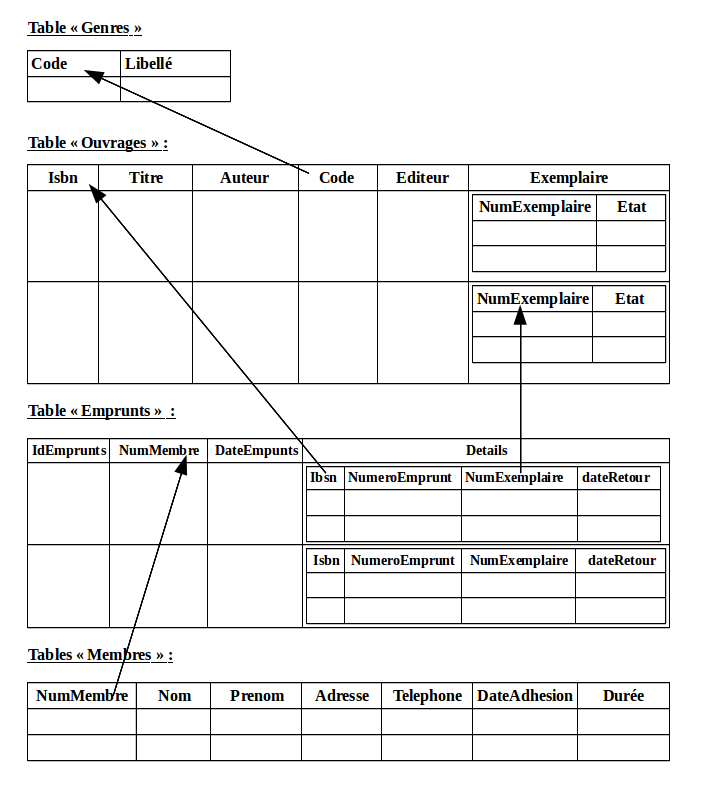
\includegraphics[scale=0.57]{object3.png} \\

La table "Exemplaires" pourrait être intégrée à la table "Ouvrages" et la table "Détails" pourrait être intégrée à la table "Emprunts", toutes deux en tant que collection. On pourrait choisir de ne pas modifier la table "Membres" ou, du moins, faire appel à la table "Emprunts" en tant que pointeur dans la table "Membres". Il serait peu judicieux d'imbriquer la table "Membres" dans la table "Emprunts", puisqu'un membre peut emprunter plusieurs fois, à des dates différentes. Une grande et même table imbriquant les deux générerait de la redondance dans les données. \\
La table "Genres" est difficilement modifiable, si on intégrait celle-ci à a table "Ouvrages", il y aurait alors des redondances dans les données.



\end{document} 